\documentclass[conference]{IEEEtran}
\usepackage{graphicx}
\usepackage{booktabs}
\usepackage{amsmath,amssymb}
\usepackage{cite}
\usepackage[hidelinks]{hyperref}
\graphicspath{{figures/}}

\begin{document}

\title{The Shared/Routed Split in Small Mixture-of-Experts\\ Models Is a Design Choice, Not a Diagnosis}

\author{\IEEEauthorblockN{AUTHOR NAMES}
\IEEEauthorblockA{AFFILIATION\\ email@domain}}

\maketitle

\begin{abstract}
Small Mixture-of-Experts language models built with an always-on shared expert appear to
under-use their routed experts: removing the entire routed branch costs little in perplexity,
while removing the single shared expert costs a great deal. We show that this asymmetry reflects
optimization dynamics and architectural proportion rather than any property of the computation
being performed. Across models of 58M to 436M parameters trained on a domain-labelled corpus, the
imbalance is transient: in the 134M reference model the two branches equalize by roughly 300M
tokens, while a twice-deeper model remains shared-dominated longer. We trace the imbalance to a
gradient-exposure race in which the shared expert, updated on every token, out-competes routed
experts updated on a $k/E$ fraction of them. The race is causally controllable: slowing the shared
expert reallocates computation to the routed branch at no cost in perplexity, and the reallocation
persists to the end of our budget even when the handicap covers only the first tenth of training.
Where the branches settle is governed jointly by their relative width and by the routing
granularity, not by the number of experts. At fixed routing, an eightfold change in the shared
expert's width moves the shared branch's share of ablation impact from 0.28 to 0.81 at essentially
unchanged perplexity; at identical widths, top-1 and top-4 routing land at 0.97 and 0.17; and
single-expert routing never engages the routed branch at any width we tested.
\end{abstract}

\begin{IEEEkeywords}
mixture of experts, training dynamics, sparse models, language models, expert specialization
\end{IEEEkeywords}

\section{Introduction}

Mixture-of-Experts (MoE) layers replace a dense feed-forward block with a router that dispatches
each token to a small number of experts. The DeepSeekMoE design~\cite{dai2024deepseekmoe} adds an
always-on \emph{shared} expert beside the \emph{routed} ones, on the intuition that the shared
expert absorbs computation common to all tokens and thereby frees the routed experts to
specialize. Because small MoEs are inexpensive to train and every token can be labelled, they have
become a common testbed for studying how experts divide work.

In this small-scale regime a striking observation recurs. Ablating the entire routed branch barely
moves held-out perplexity, whereas ablating the lone shared expert degrades it severely. Read at
face value it says the routed experts are nearly useless, inviting two explanations,
over-parametrization on the routed side or suppression by the shared expert, both of which blame
the architecture.

We argue that neither is right, and that the imbalance says almost nothing about what the
computation requires. It is instead the joint product of two things that have no obvious
connection to the task: how quickly each branch is trained, and how wide each branch is. The
apparent redundancy is transient, disappearing once the model has seen a few hundred million
tokens. Its cause is a race for gradient signal that the shared expert wins by construction, and
that a single learning-rate multiplier hands to the routed branch instead, at no cost in
perplexity. Applying the multiplier over the first tenth of training suffices; once the race is
decided, the allocation persists long after the handicap is removed. Where the two branches
finally come to rest is set jointly by their relative width and by the routing granularity, and
not, as the mechanism naively suggests, by the number of routed experts: holding the routed branch
identical down to its parameter shapes and varying only the shared expert's width moves the shared
branch's share of ablation impact from 0.28 to 0.81, while at identical widths top-1 and top-4
routing land at 0.97 and 0.17. Granularity is the one lever among these that has to be paid for,
and single-expert routing marks its degenerate end, never engaging the routed branch at all.

Two senses of ``redundant'' must be kept apart: a branch is ablation-redundant if removing it is
cheap, functionally redundant if the other could have carried its work. Our results split them.
With enough training the routed experts are not ablation-redundant at all, while the branches prove
close to interchangeable in where the computation may sit; this paper's diagnostic warning concerns
the first sense, its design freedom the second.

Taken together these results reframe the shared/routed split as a largely free design choice.
Among configurations of comparable size, held-out perplexity varies by less than 0.1 while the
branch split spans 0.25 to 0.81, so a practitioner may place the computation more or less where
they wish. That
freedom matters whenever the routed experts are themselves the object of interest, as they are in
interpretability work, expert pruning, and modular editing~\cite{muennighoff2024olmoe,lu2024notall}, and it means that a diagnosis of
expert redundancy drawn from an undertrained checkpoint is not merely imprecise but misleading.
Whether experts so engaged also become better objects of study turns out to depend on which lever
is used: widening the routed branch relative to the shared one more than doubles their domain
specialization, whereas the learning-rate control does not reliably move it at all.

\section{Related Work}

Conditional computation through a sparsely gated MoE layer was introduced by Shazeer et
al.~\cite{shazeer2017outrageously} and scaled by GShard~\cite{lepikhin2021gshard} and Switch
Transformer~\cite{fedus2022switch}, which popularized the auxiliary load-balancing loss in the
form we use; ST-MoE~\cite{zoph2022stmoe} added the router $z$-loss for stability. Our reference configuration is top-2, in the style of Mixtral~\cite{jiang2024mixtral}, and
Section~\ref{sec:topk} varies that choice.

The always-on shared expert originates with DeepSeekMoE~\cite{dai2024deepseekmoe} and carries
through DeepSeek-V2 and V3~\cite{deepseekv2,deepseekv3} and further open families such as
Qwen2~\cite{qwen2technical}, motivated by the argument that isolating common knowledge in a shared
branch lets the routed experts specialize more sharply. DeepSeekMoE pairs it with a second
argument, that finer expert segmentation sharpens specialization; Section~\ref{sec:topk} tests a
controlled analogue of that manipulation in isolation. Both arguments concern what the branches
represent. Our results concern how the branches are trained and proportioned, and they suggest
that at small scale the latter consideration dominates.

Observational studies report that experts organize more by token identity and surface form than by
topic~\cite{jiang2024mixtral,muennighoff2024olmoe}; these characterize training's outcome, while we
add a causal probe and a training-dynamics cause.

The mechanism instantiates a broader phenomenon: the early phase of training commits a network to
structure later training refines rather than revisits~\cite{achille2019critical,frankle2020early},
a phase whose routing instability motivated StableMoE~\cite{dai2022stablemoe} and whose expert
divergence has recent theory~\cite{chen2022understanding}. Our hysteresis experiment tests that
commitment directly.

\section{Experimental Setup}

\paragraph{Model} The model is a decoder-only MoE implemented from scratch in PyTorch, with Multi-head Latent
Attention~\cite{deepseekv2}, RoPE~\cite{su2021roformer} and RMSNorm~\cite{zhang2019rmsnorm}. Each
layer carries $E$ routed experts and one shared expert with top-$k$ routing. The reference
configuration has $E=8$, $k=2$, 8 layers, hidden size 512, context 512 and 134M parameters; every
expert, routed or shared, has intermediate width 1024. Section~\ref{sec:ratio} varies the two
widths independently and writes them $I$ per routed expert and $I_{\mathrm{shared}}$ for the shared
one. Configurations range from 58M to 436M parameters. All runs use AdamW ($\beta_1{=}0.9$,
$\beta_2{=}0.95$, decay 0.1), cosine to zero after 1500 warmup steps, batch 64 at length 512, peak
learning rate $3\times10^{-4}$, load-balancing coefficient $10^{-2}$, router $z$-loss $10^{-3}$,
bfloat16, capacity factor 1.25 in training and none in analysis; 30\,000 steps is 983M tokens, on
one RTX A6000.

\paragraph{Data} Pre-training streams three token-labelled corpora: FineWeb-Edu~\cite{penedo2024fineweb}
(60\%), Cosmopedia-v2~\cite{benallal2024cosmopedia} (25\%) and OpenWebMath~\cite{paster2023openwebmath}
(15\%), tokenized with a 32k vocabulary and packed to 512 tokens. Held-out evaluation uses a
skip-offset of the same streams rather than a fully disjoint split; absolute perplexities may
therefore be flattered by near-duplication, but every claim below rests on differences between
conditions evaluated on the identical stream, not on levels.

\paragraph{Measuring where the computation lives} We ablate a whole branch, either all routed
experts or the shared expert, and record the increase in held-out perplexity. Single-expert
ablation is uninformative under top-$k$ routing, since the router reroutes to the survivors. We
summarize the two measurements by the shared branch's share of total ablation impact,
\begin{equation}
s = \frac{\Delta_{\text{shared}}}{\Delta_{\text{shared}} + \Delta_{\text{routed}}},
\end{equation}
so that $s=0.5$ denotes branches of equal importance and $s\rightarrow1$ a shared-dominated model.
Almost every trajectory we measured dips to a minimum and then rises slowly, the exceptions being
the top-1 configurations of Section~\ref{sec:topk}, which decline monotonically and never leave
shared dominance; we therefore report the minimum reached over the trajectory and, where the
endpoint matters, the value at 983M tokens. Every configuration for which we ran a second seed or
a replicate run (eight, across both depths) put the spread on $s$ at 0.03 or less, an order of
magnitude below the effects discussed below.

\paragraph{Reference points} A dense FFN at the reference model's active width (58M parameters)
reaches perplexity 3.11 at 983M tokens against the reference MoE's 3.00, and deleting the shared
expert costs 0.03: the architecture earns its inactive parameters here, while the always-on branch
is worth about its parameter share, its distinctive value being organizational
(Section~\ref{sec:spec}).

\paragraph{Is $s$ measuring computation, or output norm?} Zero-ablation perturbs the residual
stream by an amount that scales with the removed branch's output norm, and both levers studied
below modulate that norm. Table~\ref{tab:valid} validates the statistic. Substituting each ablated
branch's per-layer mean output for zeros reproduces $s$ within 0.04 everywhere, ordering unchanged.
The norm share dissociates from $s$ in both directions --- under top-1 the routed branch holds
24\% of the norm and 3\% of the impact; under a slowed shared expert the shared branch holds 32\%
of the norm and 10\% of the impact --- so $s$ is no norm readout. And a fixed scalar of 2 or 0.5 on
the shared output moves the split by at most 0.07 at flat perplexity, the network \emph{absorbing}
it by rescaling weights until the trained norm share returns within 0.01 of baseline, where width
manipulations, which no rescaling absorbs, move $s$ by 0.35. Contribution norm follows function
here; it does not set it.

\begin{table}[t]
\centering
\caption{Measurement validity. $s_0$ zero-ablation, $s_\mu$ mean-ablation, $\nu$ norm share, at
983M tokens (learning-rate rows at 491M). The ordering is identical under both ablations, and
$\nu$ reaches neither extreme.}
\label{tab:valid}
\begin{tabular}{lccc}
\toprule
configuration & $s_0$ & $s_\mu$ & $\nu$ \\
\midrule
shared LR $\times0.1$        & 0.10 & 0.11 & 0.32 \\
top-4                        & 0.19 & 0.21 & 0.44 \\
$I_{\mathrm{shared}}{=}512$    & 0.34 & 0.35 & 0.45 \\
$I{=}2048$                   & 0.40 & 0.43 & 0.48 \\
scalar $\times2$             & 0.43 & 0.48 & 0.52 \\
scalar $\times0.5$           & 0.46 & 0.53 & 0.50 \\
reference                    & 0.50 & 0.54 & 0.51 \\
shared LR $\times0.3$        & 0.52 & 0.55 & 0.45 \\
$I{=}256$                    & 0.80 & 0.81 & 0.61 \\
$I_{\mathrm{shared}}{=}4096$   & 0.82 & 0.86 & 0.67 \\
top-1                        & 0.97 & 0.97 & 0.76 \\
\bottomrule
\end{tabular}
\end{table}

\section{Branch Importance Is a Function of Training Tokens}
\label{sec:obs}

We train the reference model for 983M tokens with four seeds and measure branch importance at
every checkpoint (Fig.~\ref{fig:traj}).

\begin{figure}[t]
\centering
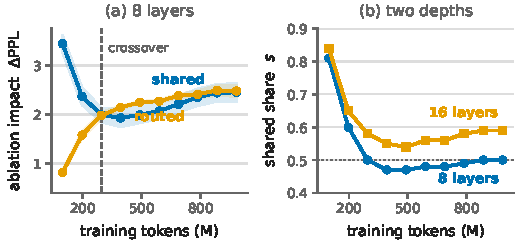
\includegraphics[width=\linewidth]{fig1_trajectory.pdf}
\caption{Ablation impact of removing the shared expert against all eight routed experts, over a
four-seed trajectory at constant batch size. Bands are $\pm1$ standard deviation. The branches
cross to equal importance by roughly 295M tokens.}
\label{fig:traj}
\end{figure}

At 98M tokens removing the shared expert costs $+3.44\pm0.17$ perplexity against $+0.82\pm0.03$
for the whole routed branch, so the shared expert accounts for 81\% of the ablation impact and the
routed experts do look close to redundant. This is the regime in which many pilot studies operate, including
our own earlier experiments. By 295M tokens the branches have equalized ($+1.99$ against $+1.98$, $s=0.50$) and they remain so
through 983M ($+2.45\pm0.18$ against $+2.48\pm0.11$), while perplexity falls from 4.18 to 3.00; routed specialization grows in parallel, with the expert--domain normalized mutual
information (NMI, defined in Section~\ref{sec:spec}) rising from 0.0008 at initialization to
0.0174. All four seeds follow the same trajectory with tight error bars.

The practical reading is narrow but firm. Branch importance is not a property of the architecture
that can be measured once; it is a function of how much data the model has seen. Conclusions about
routed redundancy drawn below a few hundred million tokens do not survive further training, and
the effect is large enough that the sign of a comparison can change.

\section{A Gradient-Exposure Race}
\label{sec:mech}

Why should the shared expert lead at all? The asymmetry is present in the update rule before it is
present in the weights. Writing the block output on token $t$ as
\begin{equation}
y_t = f_{\mathrm{sh}}(x_t) + \sum_{e\in\mathrm{topk}(t)} g_{t,e}\, f_e(x_t),
\end{equation}
with $f_{\mathrm{sh}}$ the shared expert, $f_e$ the routed ones and $g_{t,e}$ the router's gate
weight for expert $e$ on token $t$, a batch of $N$ tokens delivers gradient from
all $N$ of them to the shared parameters but from only about $Nk/E$ to any given routed expert.
Under a common learning rate the shared expert therefore accumulates roughly $E/k$ times more
effective updates per parameter during the early phase, when gradients are large and the
allocation of work is still plastic. The residual stream compounds this: it routes common
computation to whichever submodule reduces loss fastest, which further starves the routed experts
of useful gradient.

This account makes two predictions. Reducing the shared expert's learning rate should let the
routed experts capture computation earlier, and the crossover should scale with $E/k$. The first
holds; the second does not, and Section~\ref{sec:ratio} is devoted to what replaces it.

\subsection{A learning-rate handicap decides the race}

We place the shared expert's parameters in their own optimizer group at $\mathrm{lr}\times m$ and
leave everything else untouched. Table~\ref{tab:lr} reports the state at 98M tokens, deep in the
regime where the baseline looks shared-dominated.

\begin{table}[t]
\centering
\caption{Shared-expert learning-rate multiplier, two seeds, measured at 98M tokens.}
\label{tab:lr}
\begin{tabular}{lrrrr}
\toprule
$m$ & remove shared & remove routed & $s$ & PPL \\
\midrule
1.0 (baseline) & $+3.46\pm0.12$ & $+0.85\pm0.01$ & 0.80 & 4.16 \\
0.3            & $+2.48\pm0.02$ & $+1.94\pm0.00$ & 0.56 & 4.10 \\
0.1            & $+0.72\pm0.08$ & $+4.46\pm0.11$ & 0.14 & 4.10 \\
\bottomrule
\end{tabular}
\end{table}

\begin{figure}[t]
\centering
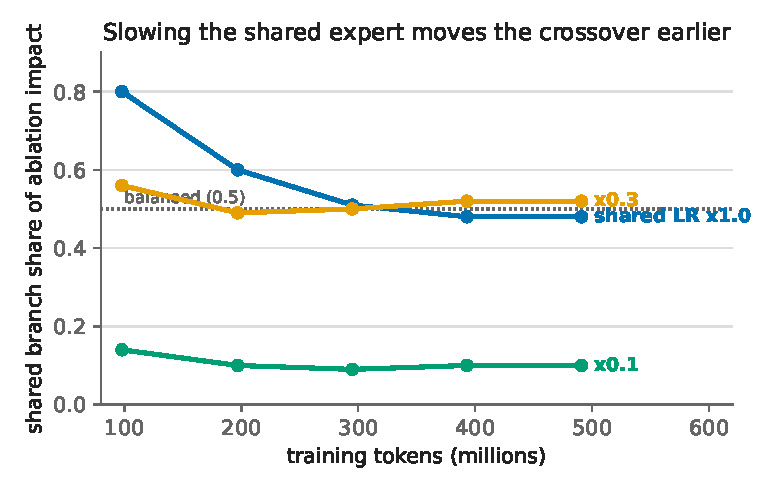
\includegraphics[width=\linewidth]{fig2_mechanism.pdf}
\caption{Shared branch share against training tokens for three shared-expert learning-rate
multipliers, two seeds. Slowing the shared expert moves the crossover earlier, and the shift grows
with the strength of the handicap.}
\label{fig:lr}
\end{figure}

Slowing the shared expert makes the routed branch load-bearing far earlier: a fivefold increase in
routed ablation impact at a fixed token budget, shifting the crossover from roughly 295M tokens to
below 200M at $m=0.3$ and to before training settles at $m=0.1$; Fig.~\ref{fig:lr} traces the full
trajectories. The effect is monotone and dose-dependent. It refutes the hypothesis that routed experts simply mature on their own schedule;
they were being out-competed.

The multiplier runs use a 15\,000-step schedule; one tenth in, where Table~\ref{tab:lr} is read,
the schedules' learning rates differ by under three percent, so the contrast is the multiplier
(the baseline row is the reference run over two seeds, hence its last-digit difference from the
four-seed reading above). Held-out perplexity is unchanged across conditions, marginally better when
the shared expert is slowed: it is not necessary for the computation it performs in the baseline.
The model puts the work there because that is where it is learned fastest, not because that is
where it belongs.

\subsection{The control holds at greater depth}

A mechanism that depended on our particular depth would be of little interest, so we repeat the
sweep on a model of twice the depth, 16 layers and 251M parameters. The control reproduces almost
exactly. At 98M tokens the shared share falls from 0.82 to 0.64 to 0.21 across the same three
multipliers, against 0.80, 0.56 and 0.14 at 8 layers, and perplexity is again unchanged. The right
panel of Fig.~\ref{fig:scale} places the two depths side by side (baseline 0.82 in the sweep
replicate against 0.84 in the long-schedule run, within the Section~III spread).

What depth does change is the timing of the unaided crossover, and it changes it in the direction
that makes the phenomenon more treacherous rather than less. The 8-layer baseline crosses to equal
importance at roughly 295M tokens and stays there. The 16-layer baseline never crosses within our
budget: it reaches a minimum of 0.54 near 491M tokens and then drifts back up to 0.59 by 983M, as
the left panel of Fig.~\ref{fig:scale} shows. That baseline is a single run, though its sweep-side
replicate above tracks it to within 0.02 over their common range. Our deeper model therefore
remains in the shared-dominated regime considerably longer -- one depth pair, but in the direction
the mechanism predicts, since more residual capacity gives the shared expert's head start more
room to compound. It also means the
warning of Section~\ref{sec:obs} grows stronger with scale rather than weaker: the larger the
model, the longer an observer will be able to look at it and conclude, wrongly, that its routed
experts are redundant. We emphasize that this concerns the crossover reached without intervention;
the following subsection shows the deeper model can be driven well past balance and kept there.

\begin{figure*}[t]
\centering
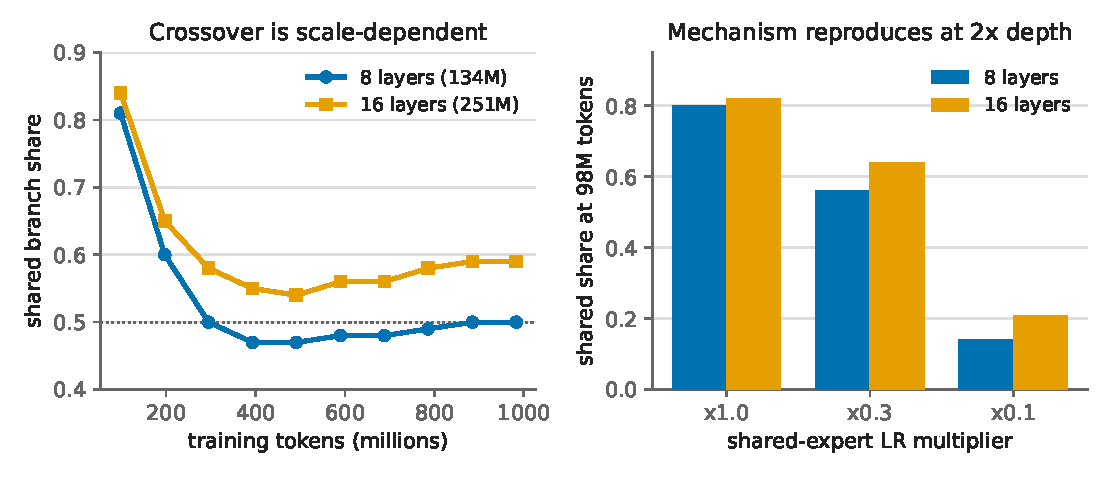
\includegraphics[width=0.86\textwidth]{fig5_scale.pdf}
\caption{Left: shared branch share against tokens for the unaided baseline at two depths. The
8-layer model crosses to equal importance; the 16-layer model approaches but does not, within 983M
tokens. Right: the learning-rate control reproduces at twice the depth, lowering the share
dose-dependently at both scales.}
\label{fig:scale}
\end{figure*}

\subsection{A temporary handicap is enough}

If the split is decided by an early race, a handicap covering only that race should suffice, and
the allocation should not revert once it is lifted. We test this on the 16-layer model by ramping
$m$ linearly from 0.1 back to 1.0 by a chosen step, after which every parameter trains at the base
rate. Fig.~\ref{fig:dose} shows the outcome for four ramp endpoints.

\begin{figure*}[t]
\centering
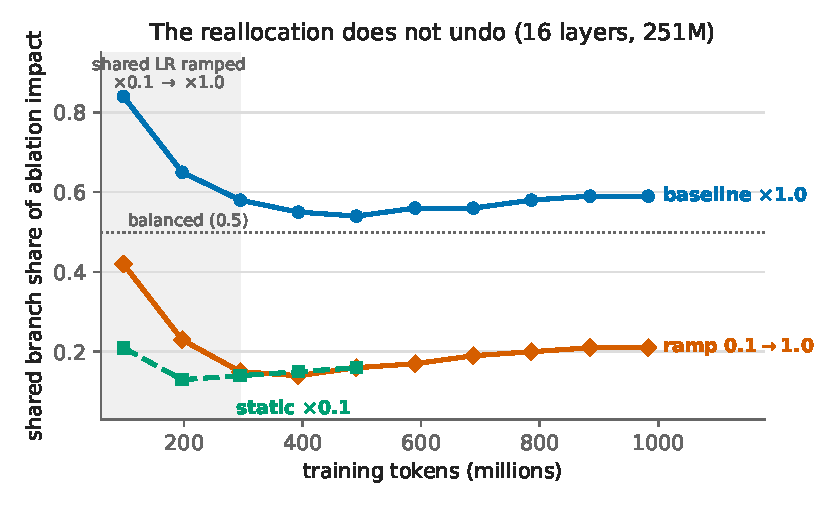
\includegraphics[width=0.86\textwidth]{fig6_hysteresis.pdf}
\caption{Left: shared branch share against training tokens at 16 layers, for four handicap
durations; the tick marks the point at which each handicap was lifted. Right: the resulting
dose-response, final share against how long the handicap was held, with the never-released limit
as a dashed reference. Every ramped condition ends within 0.01 perplexity of the others.}
\label{fig:dose}
\end{figure*}

The reallocation does not undo. Once the handicap is removed the share stays near where the
handicap left it rather than returning to the baseline trajectory, and the shared branch reasserts
itself only slowly. The response is monotone in the duration of the handicap: the share at 983M
tokens is 0.33, 0.26, 0.21 and 0.19 for handicaps lifted at 98M, 197M, 295M and 491M tokens
respectively, against 0.59 with no handicap at all and 0.14 for a handicap never lifted. Final
perplexities are 2.88, 2.88, 2.88 and 2.89, against 2.90 for the baseline and 2.91 when the
handicap is never released.

Three features of that curve matter more than its monotonicity. A brief handicap already does much
of the work: lifting it after 98M tokens, one tenth of the budget, reaches 0.33, which is more than
half of the distance from the baseline to the never-released limit. The increments shrink (0.07,
0.05, 0.02), yet the never-released limit at 0.14 sits a further 0.05 below the longest ramp: the
response flattens without plateauing in our range. And releasing the handicap is not merely harmless but marginally preferable:
every ramped condition ends at 2.88 or 2.89, better than both the untouched baseline and the permanently
handicapped run, which is the only condition here that is worse than doing nothing. The knob is
thus a schedule intervention rather than a standing tax on the shared expert, which is what a
race-then-commit dynamic predicts, since what wins the early race is what the residual stream
subsequently builds upon.

We replicated the 295M endpoint with a second seed and obtained the same summary statistics, a minimum of 0.14 and 0.21 at 983M tokens. The other four
conditions are single-seed, and the sweep covers one depth and one handicap strength, so we report
the shape of the dependence rather than a functional law.

\section{What Sets Where the Split Lands}
\label{sec:ratio}

The mechanism explains why the shared expert leads and shows that the lead can be reversed. It does
not say where the split comes to rest, and the natural prediction from the gradient-exposure
argument, that the resting point should follow $E/k$, turns out to be wrong. We assemble eleven
8-layer configurations, all at top-2 routing: the five runs of Table~\ref{tab:contrast}, a
capacity-matched sweep over expert count described below ($E\cdot I$ held at 8192 for
$E\in\{4,8,16,32\}$), and three runs from an earlier sweep at ratio 1.0 ($E=4$, 16 and 32 at
$I=I_{\mathrm{shared}}=1024$, 83M to 436M parameters). Ten trained to 983M tokens; the earlier
$E=4$ run stopped at 491M with its share flat from 295M on. Across all eleven, expert count is
nearly irrelevant and the ratio of the two branches' widths orders every run.
Section~\ref{sec:topk} then asks what happens when the routing itself is changed.

\begin{table}[t]
\centering
\caption{Two disentangling contrasts, both at $E{=}8$, $k{=}2$. Values are the minimum shared share
reached over the trajectory.}
\label{tab:contrast}
\begin{tabular}{lrrr}
\toprule
\multicolumn{4}{l}{\emph{Varying routed width}, $I_{\mathrm{shared}}=1024$}\\
$I$        & 256    & 1024   & 2048 \\
$s_{\min}$ & 0.79   & 0.47   & 0.37 \\
$s$ at 983M & 0.80  & 0.50   & 0.40 \\
parameters & 58.2M  & 133.7M & 234.4M \\
\midrule
\multicolumn{4}{l}{\emph{Varying shared width}, $I=1024$; routed branch identical}\\
$I_{\mathrm{shared}}$ & 512 & 1024 & 4096 \\
$s_{\min}$ & 0.28   & 0.47   & 0.81 \\
$s$ at 983M & 0.34  & 0.50   & 0.82 \\
parameters & 127.4M & 133.7M & 171.5M \\
\bottomrule
\end{tabular}
\end{table}

Table~\ref{tab:contrast} isolates the two candidates. Both contrasts hold $E=8$ and $k=2$ fixed, so
expert count, routing and per-expert gradient share are constant throughout. The second contrast is
the decisive one: with $I$ pinned at 1024 the routed branch is identical across the three runs, the
same number of experts of the same width receiving the same routed capacity $k\cdot I = 2048$, and
yet the split moves by 0.53. Whatever governs the resting point, it is not the absolute capacity of
the routed branch.

\begin{figure*}[t]
\centering
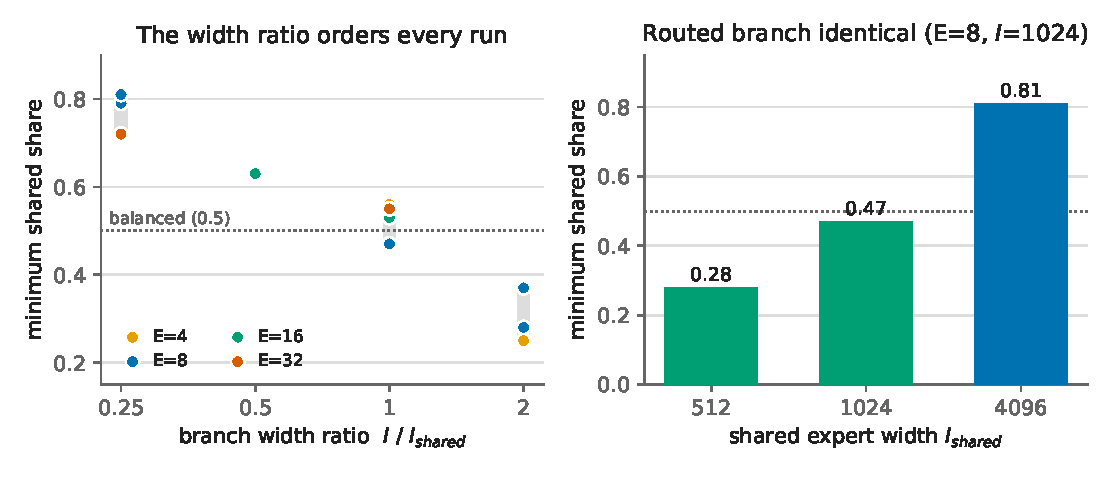
\includegraphics[width=0.86\textwidth]{fig3_ratio.pdf}
\caption{Left: minimum shared share against the branch width ratio, one point per configuration,
coloured by expert count; the bands at each ratio do not overlap. Right: the decisive contrast, in
which the routed branch is identical across all three runs and only the shared expert's width
changes.}
\label{fig:ratio}
\end{figure*}

What the two contrasts share is the ratio $I/I_{\mathrm{shared}}$. Grouping every configuration by
that ratio yields bands that do not overlap, as Fig.~\ref{fig:ratio} shows: shared shares of
0.72--0.81 at ratio 0.25, 0.63 at ratio 0.5 (a single configuration), 0.47--0.56 at ratio 1.0 and
0.25--0.37 at ratio 2.0.
The ordering survives an eightfold range in ratio, an eightfold range in expert count and a
sevenfold range in parameter count.

Expert count does not explain the residual spread within a band, and it does not even act in a
consistent direction: at ratio 2.0 more experts raise the share, from 0.25 at $E=4$ to 0.37 at
$E=8$, while at ratio 0.25 more experts lower it, from 0.79 at $E=8$ to 0.72 at $E=32$. A reader
might still suspect that the sweep confounds expert count with capacity, since a naive sweep over
$E$ at fixed per-expert width grows the routed branch as it grows $E$. Holding the product
$E\cdot I$ at 8192 removes that confound and equalizes parameter counts; perplexity is then flat
across $E\in\{4,8,16,32\}$ at 2.99, 3.00, 3.00 and 3.02, while the share continues to track the
ratio that the same manipulation necessarily varies. At matched capacity, expert count is thus
close to a free parameter for perplexity, and it moves the split only within the residual spread
of a ratio band.

\subsection{Does routing granularity enter?}
\label{sec:topk}

Every configuration above uses top-2 routing, so the ordering just established is, strictly, an
ordering at fixed $k$. Because a token passes through $k$ routed experts but only one shared
expert, $k$ has an obvious claim to matter, and we test it directly by holding the widths at
$I = I_{\mathrm{shared}} = 1024$, so the width ratio is 1.0 throughout, and varying only $k$.

\begin{table}[t]
\centering
\caption{Routing granularity at fixed widths ($E{=}8$, $I{=}I_{\mathrm{shared}}{=}1024$, ratio 1.0),
two seeds each ($k{=}2$: four); perplexity and NMI at 983M tokens.}
\label{tab:topk}
\begin{tabular}{lrrr}
\toprule
$k$ & 1 & 2 & 4 \\
\midrule
$s_{\min}$              & 0.97 & 0.47 & 0.17 \\
$s$ at 983M             & 0.97 & 0.50 & 0.19 \\
final PPL               & 3.13 & 3.00 & 2.99 \\
routed domain NMI       & 0.0003 & 0.0174 & 0.0235 \\
\bottomrule
\end{tabular}
\end{table}

Table~\ref{tab:topk} shows that $k$ enters, and that it is the strongest single lever in this
study: moving from top-1 to top-4 at identical widths swings the split from 0.97 to 0.17, further
than the 0.53 obtained by quadrupling the shared expert's width. The width-ratio result of the
preceding subsections must therefore be read as holding at fixed routing, which is how we state it.

This also refines, rather than simply refutes, the $E/k$ prediction of Section~\ref{sec:mech}. That
prediction fails on the $E$ axis, as the preceding subsection showed: at a fixed width ratio,
varying $E$ from 4 to 32 leaves the split within the single band 0.47--0.56 and not even in a
consistent direction, so per-expert gradient share cannot be what governs the resting point. It
succeeds on the $k$ axis, and in the predicted
direction, since raising $k$ lowers the shared share. The asymmetry is informative. What fails is
the \emph{ratio} $k/E$; what survives is $k$ alone. The two runs below show that $k$'s effect is
not even carried by the extra width it activates, which leaves the granularity of the routing
itself, how many experts share a token, as an operative variable alongside the branch
proportion.

Unlike the width ratio, this lever is not free. Top-1 costs 0.13 in perplexity and top-4 doubles
the routed floating-point cost per token, whereas the width manipulations moved the split across
0.25 to 0.81 within a 0.07 band of perplexity. Granularity buys reallocation; it does not buy it
for nothing.

A natural repair would be a single scalar folding $k$ in, the fraction of \emph{active}
feed-forward width the shared branch represents, $\phi = I_{\mathrm{shared}}/(I_{\mathrm{shared}}
+ kI)$. Two further runs test it directly, and refute it. Both hold $k\cdot I = 2048$ and
$I_{\mathrm{shared}} = 1024$, the same active widths and the same $\phi = 0.33$ as the reference
configuration ($s_{\min} = 0.47$), and change only how the routed width is delivered: as four
experts of 512, or as one expert of 2048. If active width were sufficient, both should land near
0.47. Neither does. Four-of-512 reaches 0.29 (final perplexity 3.06 at 96M parameters), well below
the reference, so granularity acts on its own even among $k\geq2$ configurations: the same active
width delivered through more, narrower experts engages the routed branch more. At matched active
width and a fixed expert pool, this is a controlled test of DeepSeekMoE's fine-grained segmentation
argument~\cite{dai2024deepseekmoe}, and it comes out in that argument's favour, on engagement here
and on specialization in Section~\ref{sec:spec}. And one-of-2048
stays at 0.95, so top-1's collapse is not a width effect either; doubling the per-token routed
width changes essentially nothing when the router cannot mix experts.

The top-1 failure is not mysterious: with no ability to blend experts, the routed branch never
becomes a useful object at all -- ablating it costs 0.29 perplexity and its domain NMI
\emph{declines} over training toward zero -- a qualitatively different regime, consistent with
the known difficulty of single-expert routing~\cite{fedus2022switch}. What the data support is
therefore a joint statement,
not a scalar law: at fixed granularity the width proportion orders every configuration we
measured; at fixed active width, finer granularity lowers the shared share further; and
single-expert routing never engages the routed branch at any width we tested.

These results compose: the gradient race decides which branch arrives first, the branch proportion
and routing granularity where the allocation settles once it is over. The width manipulations are
reparametrizations rather than levers on quality -- shared share 0.25 to 0.81 across the seven
127M--234M configurations, perplexity 2.95 to 3.02 -- with granularity the one exception that must
be paid for.

\section{Does Reallocation Buy Specialization?}
\label{sec:spec}

The motivation for wanting routed experts engaged is usually that they are the object of study, so
it matters whether experts forced to carry more computation also organize their work more sharply.
We measure gate-weighted normalized mutual information between expert assignment and the domain
label of each token, comparing at matched training steps and, where possible, at identical routed
architecture. Fig.~\ref{fig:spec} collects the result, and it is not the simple one.

\begin{figure}[t]
\centering
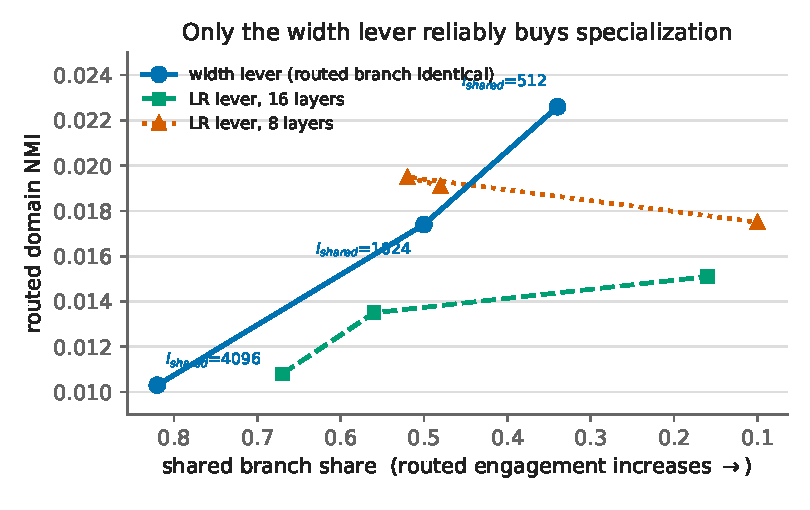
\includegraphics[width=\linewidth]{fig7_specialization.pdf}
\caption{Routed domain specialization against branch split, with routed engagement increasing to
the right; the width series is read at 983M tokens, the learning-rate series at 491M. The width
lever, whose three runs share a byte-identical routed branch, more than doubles specialization.
The learning-rate lever helps at 16 layers, where the baseline is still shared-dominated, and does
not at 8 layers, where balance has already been reached.}
\label{fig:spec}
\end{figure}

The width lever delivers. Holding $E=8$ and $I=1024$ so that the routed branch is identical across
runs and varying only $I_{\mathrm{shared}}$, domain NMI at 983M tokens rises from 0.0103 to 0.0174
to 0.0226 as the shared share falls from 0.82 to 0.50 to 0.34. That is a factor of 2.2 in
specialization obtained without touching the routed experts at all, and without cost in perplexity.
Because NMI is measured at 983M tokens, the splits quoted here are the values at that point rather
than the trajectory minima of Table~\ref{tab:contrast}, which is why the same three runs appear
with slightly different splits in the two places. The granularity runs of
Section~\ref{sec:topk} point the same way, their routed NMI rising from 0.0003 at top-1 to 0.0235
at top-4, and to 0.0301, the highest routed specialization measured anywhere in this study, when
the same active width is delivered as four experts of width 512. Nor is the gain specific to the
domain axis: across the same width trio, surface-form NMI rises from 0.118 to 0.141 and frequency
NMI from 0.039 to 0.056, with position at the control floor throughout -- every axis moves with
engagement, though the headline factor of 2.2 is domain-specific and the surface-form gain is a
more modest 1.2. Deleting the shared expert makes the same point from the other side: routed
domain NMI falls to 0.0113 without it, so the always-on branch, worth only 0.03 perplexity, makes
the routed experts more organized, not less.

The learning-rate lever does not, or not reliably. At 16 layers, measured at 491M tokens where the
baseline remains shared-dominated, slowing the shared expert raises NMI monotonically, 0.0108 to
0.0135 to 0.0151, all three points from the same 15\,000-step sweep. At 8 layers, where balance
has already been reached by then, the response is non-monotone, 0.0191, 0.0195 and 0.0175 for
$m = 1.0$, 0.3 and 0.1, ending below the baseline; this series reads the long-schedule reference
against short-schedule sweep runs, so we take from it only the absence of a reliable gain. The
dose-response series of Section~\ref{sec:mech} is similarly equivocal: NMI increases with handicap
duration among the ramped runs but the unhandicapped baseline falls inside their range rather than
below it.

The pattern these disagreements share is that specialization tracks how much the routed branch has
genuinely been trained, which rises as it takes over computation but flattens near balance and can
fall once the shared branch is starved past it. Engagement and specialization are therefore
related but distinct axes, and the distinction is practical: an experimenter who wants routed
experts that are better objects of interpretability should change the branch widths rather than
the learning rate, even though both move the split by comparable amounts. We note that domain
our 16-layer learning-rate runs are
single-seed, that we exclude comparisons across expert count because NMI grows
mechanically with the number of experts, and that every value is measured at balancing coefficient
$10^{-2}$, which suppresses domain NMI relative to unbalanced training, so the magnitudes are
conditional on that setting even though each contrast is internal to it.

\section{Discussion}

A small MoE's division of feed-forward labour is only weakly determined by the task. Two quantities
a practitioner sets freely, the branches' relative learning rate and relative width, move the split
across almost its whole attainable range while leaving perplexity within 0.1; a third, routing
granularity, moves it further at a cost the first two do not carry. The shared expert is not doing
what the routed experts could not; it is doing what it got to first, and it keeps as much as its
width allows.

Three consequences follow. The first is diagnostic. Expert redundancy cannot be assessed from a
single early checkpoint, because the measurement at 98M tokens and the measurement at 983M tokens
disagree, and deeper models remain in the misleading regime longer. Branch importance should be
reported as a trajectory. The second concerns design: our own early sweep over expert count read
as a dependence on $E$ only because routed capacity and parameter count rode along with it, and it
did not survive the matched comparisons of Section~\ref{sec:ratio}; sweeps over architecture
should fix what they are not testing. The third is prescriptive, and
Section~\ref{sec:spec} makes it sharper than we expected. A modest learning-rate handicap on the
shared expert engages the routed branch much sooner at no measured cost, and need only be applied
over the early part of training; but engagement bought that way does not reliably come with
sharper specialization. If the routed experts are wanted merely \emph{used}, either lever serves.
If they are wanted \emph{legible}, the width ratio is the one that works. The mechanism also
yields a prediction for routing families we did not test: expert-choice
routing~\cite{zhou2022expertchoice} equalizes token counts across routed experts but leaves the
shared expert's every-token exposure intact, so the race, and its learning-rate remedy, should
survive it.

Several limits bound these claims, and concern generality rather than internal validity. All
models fall between 58M and 436M parameters and see at most 983M tokens, on one data mixture and
one hardware configuration; whether the crossover and the controls persist at production scale is
the obvious next question. The width-ratio result is an ordering over an eightfold range at one
depth, not a functional form, and the granularity runs show no single scalar we tried subsumes
width and routing at once. The dose-response is replicated at one endpoint, its other points
resting on a single seed each; effect sizes there exceed the measured seed noise comfortably, but
the flattening deserves a denser sweep. Finally, our evidence is perplexity, ablation impact and
routing statistics: at this scale standard benchmarks sit near chance, so whether a reallocated
split changes downstream behaviour -- what a practitioner would ultimately want -- needs a larger
model to be answerable.

\section{Conclusion}

Routed experts in small Mixture-of-Experts models are not redundant in the ablation sense: they
are out-competed early by a shared expert that receives gradient from every token, and the outcome
is settled by the designer's choices rather than the data's demands. Slowing the shared expert
reverses it durably, the reallocation persisting to the end of our budget even when the handicap
covers only the first tenth of training. Where the split rests is then set jointly by the branches'
relative width, spanning shared shares of 0.25 to 0.81 at essentially unchanged perplexity, and by
routing granularity, the strongest lever and the only one that is not free. Where a small
Mixture-of-Experts model puts its feed-forward computation is, to a good approximation, something
the designer chooses rather than something the model discovers.

\section*{Reproducibility}

The model, the training code and the analysis toolkit, including whole-branch ablation, routing
capture and the trajectory drivers, will be released publicly upon acceptance, together with the
run configurations and the per-checkpoint measurements behind every table and figure here. Every
experiment in this paper runs on a single GPU. Two implementation defects found and fixed during
the study, a missing causal mask in the absorbed attention inference path and a broken CUDA
reduction in the load-balancing loss, are recorded in the version history that will accompany that
release; every measurement reported here postdates both fixes.

{\footnotesize
\bibliographystyle{IEEEtran}
\bibliography{references}
}

\end{document}
